\subsubsection{Example: Mnemonic decoding}

The reverse operation, translating from a human-legible form to the
numerical form, is trivial. Given, of course, that you know the format
that the mnemonic form is in and any conditions pertaining to the
particular instruction. 

Take for instance \tt{div \$t2, \$t4}, given that we know its mnemonic
representation to be on the form

\begin{lstlisting}[style=mips_lst]
div $rs, $rt
\end{lstlisting}
%$

and that due to its nature both \shamt{} and \rd{} is both zero,
together with the fact that we know its opcode and \funct{}, trivially
we substitute all those values in together with the register
addresses. Together we get

\begin{figure}[H]
  \makebox[\textwidth][c]{
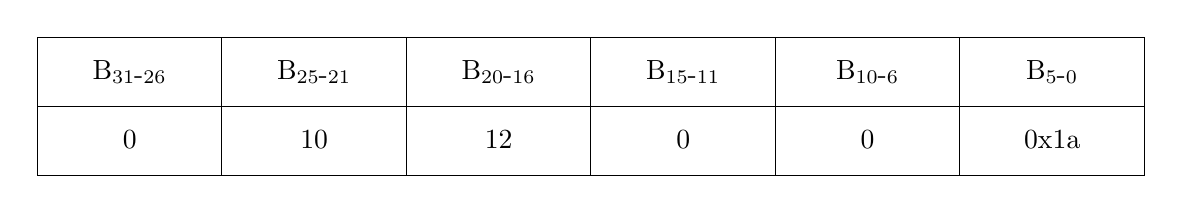
\begin{tikzpicture}[auto,
    every node/.style={rectangle, minimum height=2.5em, text centered, text width=6em, text height=1.5ex, text depth=.25ex},
    field/.style={draw}]
\matrix (m) [ampersand replacement=\&, column sep=-\pgflinewidth, row sep=-\pgflinewidth]
{
\node [field] {$\textrm{B}_{31\textrm{-}26}$}; \&
\node [field] {$\textrm{B}_{25\textrm{-}21}$}; \&
\node [field] {$\textrm{B}_{20\textrm{-}16}$}; \&
\node [field] {$\textrm{B}_{15\textrm{-}11}$}; \&
\node [field] {$\textrm{B}_{10\textrm{-}6}$}; \&
\node [field] {$\textrm{B}_{5\textrm{-}0}$}; \&
\\
\node [field] {0}; \&
\node [field] {10}; \&
\node [field] {12}; \&
\node [field] {0}; \&
\node [field] {0}; \&
\node [field] {0x1a}; \&
\\
};
\end{tikzpicture}
  }
\end{figure}

and the final translation step, and the resulting numerical
representation, is given by a sequence of bit-shift operations, in
this case the following will serve,\footnote{No operations are
  required for the zeroes.}\footnote{Notice that the shift amount (21,
  16) corresponds directly to the lower most bit of the respective fields (rs, rt)}

\begin{lstlisting}
(10 << 21) | (12 << 16) | 0x1a
\end{lstlisting}

which is equal to \tt{0x014c001a}.
